% Critic-based PPO in Flow-Factory: algorithm analysis.
% Compile: pdflatex ppo_analysis.tex (run twice for cross-references / hyperref).
% Requires: tikz, algorithm, algpseudocode, booktabs, amsmath, amsthm, hyperref.
\documentclass[11pt]{article}

\usepackage[utf8]{inputenc}
\usepackage[T1]{fontenc}
\usepackage{lmodern}
\usepackage[a4paper,margin=1in]{geometry}
\usepackage{amsmath,amssymb,amsthm,bm}
\usepackage{booktabs}
\usepackage{array}
\usepackage{enumitem}
\usepackage{caption}
\usepackage{xcolor}
\usepackage{algorithm}
\usepackage{algpseudocode}
\usepackage{tikz}
\usetikzlibrary{arrows.meta,positioning,shapes.geometric,calc,fit,backgrounds}
\usepackage[colorlinks=true,linkcolor=blue,citecolor=blue,urlcolor=teal]{hyperref}

\theoremstyle{plain}
\newtheorem{proposition}{Proposition}
\theoremstyle{remark}
\newtheorem{remark}{Remark}

% TikZ shared styles
\tikzset{
  box/.style={draw, rounded corners, align=center, minimum height=0.95cm,
              text width=3.0cm, fill=blue!5, font=\small},
  net/.style={draw, rounded corners, align=center, minimum height=0.8cm,
              text width=2.7cm, fill=teal!8, font=\small},
  state/.style={draw, circle, minimum size=0.95cm, fill=gray!8, font=\small},
  flow/.style={-{Stealth[length=2.5mm]}, thick},
}

\newcommand{\zt}{\bm{z}}
\newcommand{\E}{\mathbb{E}}
\newcommand{\R}{\mathbb{R}}

\title{\textbf{Critic-based PPO for Flow-Matching Models}\\[2pt]
\large Algorithm, Pseudocode, and Theoretical Analysis (Flow-Factory)}
\author{Flow-Factory}
\date{\today}

\begin{document}
\maketitle

\begin{abstract}
This note documents the critic-based Proximal Policy Optimization (PPO) trainer in
Flow-Factory (\texttt{trainer\_type: ppo}). It is a \emph{coupled} actor--critic
algorithm: it reuses the same SDE rollout and per-step log-probability machinery as
GRPO, but replaces GRPO's single, group-normalized advantage (broadcast to every
denoising step) with a learned, timestep-conditioned \emph{value critic} and
Generalized Advantage Estimation (GAE), giving fine-grained per-step credit
assignment. We formalize denoising as a finite-horizon MDP, give the data-flow
diagram, pseudocode, and a short theoretical analysis (variance reduction, GAE
bias--variance, the clipped surrogate). We close with a detailed comparison to
\emph{Explicit Critic Guidance for Aligning Diffusion Models}
(\href{https://arxiv.org/abs/2605.27736}{arXiv:2605.27736}), which makes the
diffusion backbone its own value function---precisely the ``backbone-critic''
variant Flow-Factory evaluated and deferred.
\end{abstract}

\tableofcontents

\section{Introduction and Motivation}
\label{sec:intro}

Flow-Factory fine-tunes flow-matching / diffusion models with online RL against
(typically non-differentiable) reward models. The default algorithm, GRPO, treats a
whole denoising rollout as a single ``action'': it computes one scalar advantage per
sample from \emph{group-relative} reward normalization and broadcasts it to all
training timesteps. This is simple and strong, but has two structural limitations:

\begin{enumerate}[leftmargin=1.4em]
  \item \textbf{No per-step credit.} Every denoising step in a trajectory shares the
  same advantage, so the gradient cannot distinguish which steps were responsible
  for a high/low reward.
  \item \textbf{Group-mean baseline.} The variance-reduction baseline is the per-group
  reward mean; it ignores the \emph{state} (the noisy latent), and its quality
  depends on the group size.
\end{enumerate}

Critic-based PPO addresses both by learning a state-conditioned value function
$V_\phi(\zt_s, t_s)$ over noisy latent states and forming \emph{per-step} advantages
with GAE. The contribution of this implementation is a \emph{lightweight,
model-agnostic} actor--critic that drops into the existing rollout pipeline:

\begin{itemize}[leftmargin=1.4em]
  \item an independent value critic that consumes the full generation latent at any
  layout (conv / packed / video) and is built eagerly from the channel count
  (Section~\ref{sec:critic});
  \item GAE per-step advantages with optional global whitening
  (Section~\ref{sec:gae});
  \item a PPO objective with policy-ratio clipping and value clipping, a critic
  warmup phase, and two optimizers sharing one backward
  (Section~\ref{sec:objective}).
\end{itemize}

\section{Preliminaries: Denoising as an MDP}
\label{sec:mdp}

\paragraph{SDE sampling.}
A rollout produces a trajectory of latents $\zt_0 \to \zt_1 \to \cdots \to \zt_S$,
where $\zt_0$ is initial noise and $\zt_S$ decodes to the generated image/video.
At each stochastic (SDE) step $s$ the scheduler (Flow-SDE) defines a Gaussian
transition (the \emph{policy})
\begin{equation}
\label{eq:policy}
\pi_\theta(\zt_{s+1}\mid \zt_s, t_s)
  = \mathcal{N}\!\big(\zt_{s+1};\, \bm{\mu}_\theta(\zt_s, t_s),\, \sigma_s^2 \bm{I}\big),
  \qquad \sigma_s = \texttt{std\_dev\_t}\cdot\sqrt{-\mathrm{d}t},
\end{equation}
whose mean $\bm{\mu}_\theta$ is a deterministic function of the network's velocity
prediction. The per-step log-probability $\log\pi_\theta$ is tractable and is exactly
what the scheduler returns and stores during rollout, which is the foundation of
train--inference consistency.

\paragraph{MDP.}
We treat the ordered SDE steps as a finite-horizon MDP:
\begin{center}
\begin{tabular}{ll}
\toprule
state & $s_s = (\zt_s, t_s)$ (noisy latent + scheduler timestep)\\
action & $a_s = \zt_{s+1}$ (the sampled next latent)\\
policy & $\pi_\theta(a_s \mid s_s)$ from Eq.~\eqref{eq:policy}\\
reward & $r_s = R\cdot\mathbb{1}[s = S{-}1]$, with terminal $R=\sum_k w_k\, r_k(\text{decode}(\zt_S))$\\
value & $V_\phi(\zt_s, t_s)$, terminal $V(\zt_S)\equiv 0$\\
\bottomrule
\end{tabular}
\end{center}

The reward is \emph{terminal only}: it is the (weighted) reward-model score of the
final decoded sample, received on the last SDE transition. Figure~\ref{fig:mdp}
illustrates the episode.

\begin{figure}[h]
\centering
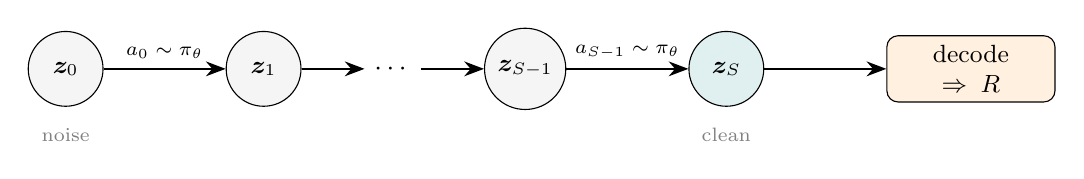
\begin{tikzpicture}[node distance=1.55cm]
  \node[state] (z0) {$\zt_0$};
  \node[state, right=of z0] (z1) {$\zt_1$};
  \node[right=0.8cm of z1] (dots) {$\cdots$};
  \node[state, right=0.8cm of dots] (zS1) {$\zt_{S-1}$};
  \node[state, right=of zS1, fill=teal!12] (zS) {$\zt_S$};
  \node[draw, rounded corners, right=of zS, fill=orange!12, font=\small, text width=1.9cm, align=center] (rew) {decode\\ $\Rightarrow R$};
  \draw[flow] (z0) -- node[above,font=\scriptsize]{$a_0\sim\pi_\theta$} (z1);
  \draw[flow] (z1) -- (dots);
  \draw[flow] (dots) -- (zS1);
  \draw[flow] (zS1) -- node[above,font=\scriptsize]{$a_{S-1}\sim\pi_\theta$} (zS);
  \draw[flow] (zS) -- (rew);
  \node[below=0.15cm of z0, font=\scriptsize, gray] {noise};
  \node[below=0.15cm of zS, font=\scriptsize, gray] {clean};
\end{tikzpicture}
\caption{Denoising rollout as a finite-horizon MDP. The policy is the per-step SDE
Gaussian transition; the reward is terminal (on the decoded final latent $\zt_S$).
The critic estimates $V_\phi(\zt_s,t_s)$ at every step.}
\label{fig:mdp}
\end{figure}

\section{From GRPO to Critic-based PPO}
\label{sec:grpo-vs-ppo}

\paragraph{GRPO.}
For a group $g$ of $K$ rollouts sharing a prompt, GRPO assigns each sample the same
advantage at \emph{every} step:
\begin{equation}
A^{\mathrm{GRPO}}_i \;=\; \frac{R_i - \operatorname{mean}_{j\in g}(R_j)}{\operatorname{std}(R)},
\qquad A^{\mathrm{GRPO}}_{i,s} = A^{\mathrm{GRPO}}_i \;\; \forall s.
\end{equation}

\paragraph{PPO.}
Critic-based PPO instead learns $V_\phi$ and forms per-step advantages by GAE
(Section~\ref{sec:gae}). The baseline is now state-aware ($V_\phi(\zt_s,t_s)$ rather
than a group mean), and credit is distributed per step. Table~\ref{tab:grpo-ppo}
summarizes the structural difference; everything else (rollout, per-step
log-probabilities, SDE dynamics, optional KL-to-reference) is shared.

\begin{table}[h]
\centering
\small
\begin{tabular}{p{3.4cm} p{5.2cm} p{5.2cm}}
\toprule
 & \textbf{GRPO} & \textbf{Critic-based PPO} \\
\midrule
Advantage & one scalar / sample, broadcast & per-step $A_s$ via GAE \\
Baseline & per-group reward mean & learned $V_\phi(\zt_s, t_s)$ \\
Extra parameters & none & lightweight value critic + its optimizer \\
Reward normalization & group-relative (mean/std) & none on $R$; advantages whitened \\
Per-epoch hook order & \multicolumn{2}{l}{\texttt{sample()} $\to$ \texttt{prepare\_feedback()} $\to$ \texttt{optimize()}} \\
\bottomrule
\end{tabular}
\caption{GRPO vs.\ critic-based PPO. Only the credit-assignment / baseline differs.}
\label{tab:grpo-ppo}
\end{table}

\section{Algorithm and Data Flow}
\label{sec:algo}

Figure~\ref{fig:pipeline} shows the per-epoch data flow. The trainer reuses
\texttt{generate\_samples} for rollout, then computes \emph{old} values with the
current critic (no grad), runs GAE, stores per-step targets on each sample, and
finally optimizes.

\begin{figure}[h]
\centering
\resizebox{\textwidth}{!}{%
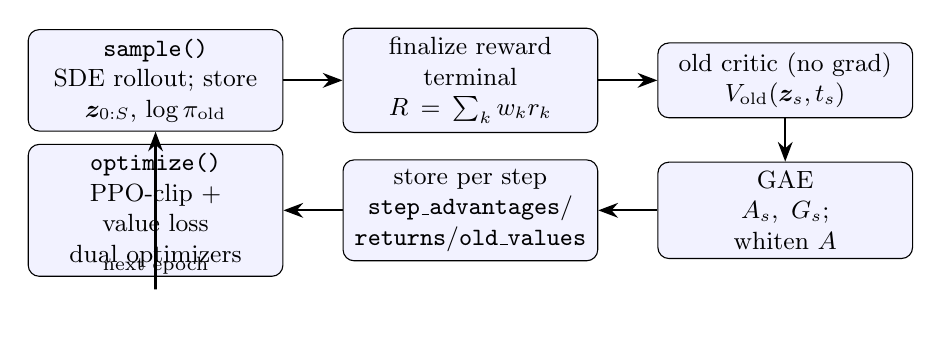
\begin{tikzpicture}[node distance=0.55cm and 0.75cm]
  \node[box] (sample) {\texttt{sample()}\\ SDE rollout; store\\ $\zt_{0:S}$, $\log\pi_{\mathrm{old}}$};
  \node[box, right=of sample] (reward) {finalize reward\\ terminal $R=\sum_k w_k r_k$};
  \node[box, right=of reward] (oldv) {old critic (no grad)\\ $V_{\mathrm{old}}(\zt_s,t_s)$};
  \node[box, below=of oldv] (gae) {GAE\\ $A_s,\ G_s$;\\ whiten $A$};
  \node[box, left=of gae] (store) {store per step\\ \texttt{step\_advantages}/\\ \texttt{returns}/\texttt{old\_values}};
  \node[box, left=of store] (opt) {\texttt{optimize()}\\ PPO-clip $+$ value loss\\ dual optimizers};
  \draw[flow] (sample) -- (reward);
  \draw[flow] (reward) -- (oldv);
  \draw[flow] (oldv) -- (gae);
  \draw[flow] (gae) -- (store);
  \draw[flow] (store) -- (opt);
  \draw[flow] (opt.south) to[out=-90,in=-90] node[below,font=\scriptsize]{next epoch} (sample.south);
\end{tikzpicture}%
}
\caption{Per-epoch pipeline of the PPO trainer. \texttt{prepare\_feedback()} covers
the reward$\to$old-value$\to$GAE$\to$store stages; \texttt{optimize()} does the
gradient update.}
\label{fig:pipeline}
\end{figure}

\subsection{Value critic}
\label{sec:critic}

The critic is an independent, resolution-agnostic network
(\texttt{trainers/ppo/critic.py}). Any latent layout is folded to $(B,\mathrm{seq},C)$
by moving the channel axis last (\texttt{latents\_to\_tokens} using
\texttt{resolve\_latent\_axes}); tokens are encoded, aggregated over the sequence by
\emph{learned-query multi-head attention pooling} (PMA-style, $O(\mathrm{seq})$),
concatenated with a sinusoidal timestep embedding, and mapped to a scalar
(Figure~\ref{fig:critic}). It is built eagerly in \texttt{\_initialization()} from the
channel count returned by \texttt{BaseAdapter.compute\_actual\_latent\_shape}, so it
needs no rollout to size and its checkpoint stays valid across resolutions.

\begin{figure}[h]
\centering
\resizebox{\textwidth}{!}{%
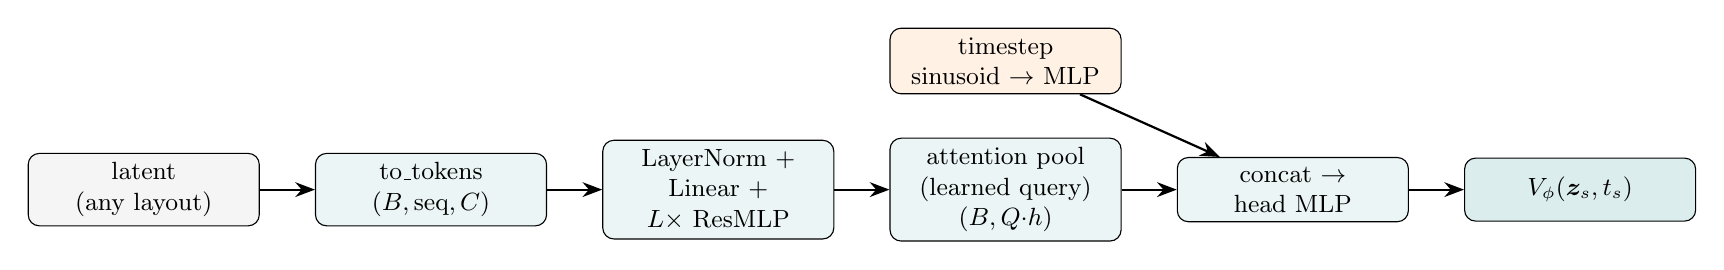
\begin{tikzpicture}[node distance=0.45cm and 0.7cm]
  \node[net, fill=gray!8] (lat) {latent\\ (any layout)};
  \node[net, right=of lat] (tok) {to\_tokens\\ $(B,\mathrm{seq},C)$};
  \node[net, right=of tok] (enc) {LayerNorm $+$\\ Linear $+$\\ $L\times$ ResMLP};
  \node[net, right=of enc] (pool) {attention pool\\ (learned query)\\ $(B,Q{\cdot}h)$};
  \node[net, above=0.55cm of pool, fill=orange!10] (time) {timestep\\ sinusoid $\to$ MLP};
  \node[net, right=of pool] (head) {concat $\to$\\ head MLP};
  \node[net, right=of head, fill=teal!14] (v) {$V_\phi(\zt_s,t_s)$};
  \draw[flow] (lat) -- (tok);
  \draw[flow] (tok) -- (enc);
  \draw[flow] (enc) -- (pool);
  \draw[flow] (pool) -- (head);
  \draw[flow] (time) -- (head);
  \draw[flow] (head) -- (v);
\end{tikzpicture}%
}
\caption{Value-critic architecture. Attention pooling keeps the network
resolution/frame agnostic (it only depends on the channel count $C$) while
preserving more information than mean/std pooling.}
\label{fig:critic}
\end{figure}

\paragraph{Backbone critic (\texttt{critic\_type=backbone}, Scheme B).}
As an alternative to the standalone net above, the critic can reuse the policy
transformer's own base weights through a \emph{separate} PEFT adapter named
\texttt{"critic"} (independent of the policy \texttt{"default"} adapter) plus a value
head on the transformer's per-token hidden features, tapped before the output
projection via \texttt{BaseAdapter.extract\_backbone\_features}. The value head joins
the single \texttt{accelerator.prepare} root (one DDP root, constraint~\#9) and is
trained by its own optimizer over the critic-LoRA $+$ value-head parameters;
\texttt{get\_trainable\_parameters()} excludes the \texttt{"critic"} adapter so the
policy optimizer never sees it. The same learned-query attention pooling as
Figure~\ref{fig:critic} aggregates the hidden features $(B,\mathrm{seq},D)$ (the
backbone feature width $D$ replaces the latent channel $C$). Limits (v1): LoRA finetune
and DDP only, and the critic and policy step together
(\texttt{critic\_update\_interval}$=$\texttt{policy\_update\_interval}); asymmetric
critic training uses periodic re-warmup bursts
(\texttt{update\_critic\_in\_optimize=false}). It costs $\sim$2x forward (a separate
critic backbone pass), so it pairs well with per-sample/bandit SDE. Supported for SD3.5.

\paragraph{State-aligned latent critic (\texttt{critic\_type=backbone\_branches}, arXiv:2605.27736).}
A paper-faithful reproduction of \emph{Explicit Critic Guidance}: the diffusion backbone is
its own timestep-conditioned value function via \texttt{DiTBranchCritic} --- per-layer
critic-attention branches at \texttt{critic\_tap\_layers} (default layers $7/15/23$), each a
learnable query token that cross-attends to that block's image tokens with QK-norm and
AdaLN timestep modulation, concatenated and mapped to a scalar by an MLP head. The branches
read the actor backbone's intermediate features (captured by forward hooks via
\texttt{BaseAdapter.extract\_block\_features} / \texttt{capture\_block\_features}) with
\emph{no} critic LoRA; the backbone is read no-grad for the critic, so the value loss trains
only the branch heads (clean actor/critic separation). The critic joins the single
\texttt{accelerator.prepare} root with its own optimizer. Limits (v1): DDP only and the critic
and policy step together; works with \texttt{lora} or \texttt{full} policy fine-tuning. Pair
with the paper preset ($\gamma=\lambda=1$, value-target clip $[-5,5]$, advantage clip
$[-10,10]$, CFG-free, $40$ SDE steps) in \texttt{examples/ppo/lora/sd3\_5/explicit\_critic.yaml}.
v1 runs a separate no-grad backbone forward for the critic value (identical detached features);
sharing the policy's forward is a deferred efficiency optimization.

\subsection{Generalized Advantage Estimation}
\label{sec:gae}

With $V_{\mathrm{old}}$ evaluated at each ordered SDE step, the TD residual and GAE
advantage are
\begin{align}
\delta_s &= r_s + \gamma\, V(\zt_{s+1}) - V(\zt_s),
  \qquad V(\zt_S)\equiv 0,\\
A_s &= \sum_{l=0}^{S-1-s} (\gamma\lambda)^l\, \delta_{s+l},
  \qquad
G_s = A_s + V(\zt_s),
\end{align}
computed by the backward recursion $A_s = \delta_s + \gamma\lambda A_{s+1}$
(\texttt{compute\_gae}). $G_s$ is the value-regression target. With a terminal-only
reward and $\gamma=\lambda=1$ this collapses to $A_s = R - V(\zt_s)$ and $G_s = R$ for
all $s$ (the critic-baselined analogue of GRPO); $\lambda<1$ trades variance for
bias. The example config uses a \emph{full, contiguous} SDE trajectory so the
bootstrap $V(\zt_{s+1})$ is the value of the actual next stored latent. Advantages are
optionally whitened across all $(\text{sample},\text{step})$ pairs and ranks via a
single all-reduce (\texttt{whiten} $\to$ \texttt{utils.dist.global\_tensor\_stats}).

\subsection{PPO objective}
\label{sec:objective}

Let $\rho_s = \exp(\log\pi_\theta(a_s\mid \zt_s) - \log\pi_{\mathrm{old}}(a_s\mid\zt_s))$
be the per-step importance ratio and $\hat A_s$ the (clamped, whitened) advantage.
The clipped objective is
\begin{align}
\mathcal{L}^{\text{pol}}
  &= -\,\E_s\!\big[\min\big(\rho_s \hat A_s,\;
       \mathrm{clip}(\rho_s, 1{+}c_-, 1{+}c_+)\,\hat A_s\big)\big],
       \label{eq:Lpol}\\
\mathcal{L}^{\text{val}}
  &= \tfrac12\,\E_s\!\big[\max\big((V_\phi - G_s)^2,\;
       (V^{\mathrm{clip}}_\phi - G_s)^2\big)\big],
       \quad V^{\mathrm{clip}}_\phi = V_{\mathrm{old}} + \mathrm{clip}(V_\phi{-}V_{\mathrm{old}}, \pm\epsilon_v),
       \label{eq:Lval}\\
\mathcal{L}
  &= \mathcal{L}^{\text{pol}} + c_v\,\mathcal{L}^{\text{val}}
       \;+\; \beta\,\mathrm{KL}(\pi_\theta \,\|\, \pi_{\mathrm{ref}}). \label{eq:Ltot}
\end{align}
As in Flow-GRPO, the ratio clip range $(c_-,c_+)$ is intentionally tiny (default
$\pm 10^{-4}$) because $\log\pi$ is a per-dimension average over a high-dimensional
Gaussian. The KL-to-reference term ($\beta=\,$\texttt{kl\_beta}) is optional and off
by default. Policy and critic use \emph{separate} backward passes (each only
traverses its own sub-graph) and each steps its own AdamW optimizer
(\texttt{optimizer}, \texttt{critic\_optimizer}); this independence is what lets
their update frequencies be decoupled (\S\ref{sec:decouple}).

\paragraph{Critic warmup as an up-front bootstrap.}
The initial critic warmup and the periodic re-warmup (\S\ref{sec:rewarmup}) share a
single critic-only path. Before the epoch loop, \textsc{BootstrapCritic} resamples
fresh rollouts and fits \emph{only} the critic until it has taken
${\sim}\,$\texttt{critic\_warmup\_steps} optimizer steps, so a value baseline is
established before any policy update (the ``value pretraining'' idea of
\cite{liang2026critic}). Unlike a warmup woven into the first epochs, this bootstrap
runs once up front and does \emph{not} freeze them: once the loop starts the policy
updates every epoch.

\subsection{Pseudocode}

The algorithm has two committed stages; both are kept for reference.
Algorithm~\ref{alg:ppo-v1} is the original formulation (commit \texttt{4bdec9d}): a single
combined loss $\mathcal{L}=c_v\mathcal{L}^{\text{val}}+\mathcal{L}^{\text{pol}}(+\beta\,\mathrm{KL})$,
one \texttt{accelerator.backward}, a shared \texttt{accumulate} window, both optimizers
stepping together at the sync boundary, and the warmup woven into the first epochs.
Algorithm~\ref{alg:ppo} is the current formulation (commit \texttt{4145161}): separate
per-network backward passes, decoupled update intervals (\S\ref{sec:decouple}), and the
warmup unified with periodic critic re-warmup (\S\ref{sec:rewarmup}).

\begin{algorithm}[H]
\caption{Critic-based PPO --- v1: combined loss, shared \texttt{accumulate} (commit \texttt{4bdec9d})}
\label{alg:ppo-v1}
\begin{algorithmic}[1]
\State $\mathcal{D} \gets \textsc{Sample}()$;\quad $\{R_i\} \gets \textsc{Reward}(\mathcal{D})$;\quad
       $\mathcal{S} \gets \mathrm{sorted}(\text{train SDE steps})$
\State $V_{\mathrm{old}} \gets V_\phi(\mathcal{D})$ (no grad);\quad $A, G \gets \textsc{GAE}$;\quad
       $A \gets \textsc{Whiten}(A)$;\quad store on samples
\For{inner epoch $=1,\dots,N$}
  \For{micro-batch $b$} \Comment{\texttt{with accumulate(model\_bundle, critic)}}
    \For{$s \in \mathcal{S}$}
      \State $V \gets V_\phi(\zt^b_s, t_s)$;\quad $\mathcal{L} \gets c_v \mathcal{L}^{\text{val}}$
      \If{$r \ge$ \texttt{critic\_warmup\_steps}}
        \State $\mathcal{L}^{\text{pol}} \gets$ Eq.~\eqref{eq:Lpol};\quad
               $\mathcal{L} \gets \mathcal{L} + \mathcal{L}^{\text{pol}} (+\,\beta\,\mathrm{KL})$
               \Comment{policy forward}
      \Else
        \State policy frozen; forward skipped
      \EndIf
      \State \textsc{Backward}$(\mathcal{L})$ \Comment{single combined backward; accelerate $\div gas$}
      \If{\texttt{sync\_gradients} at round end}
        \State clip + step \texttt{critic\_optimizer} (and \texttt{optimizer} unless warmup); zero both
      \EndIf
    \EndFor
  \EndFor
\EndFor
\end{algorithmic}
\end{algorithm}

\begin{algorithm}[H]
\caption{Critic-based PPO --- current: separate backward, decoupled frequency + re-warmup (commit \texttt{4145161})}
\label{alg:ppo}
\begin{algorithmic}[1]
\State \textbf{once, before training:} \textsc{WarmupCritic}(\texttt{critic\_warmup\_steps}) (\S\ref{sec:rewarmup}); \textbf{every} \texttt{critic\_warmup\_interval} \textbf{rounds:} \textsc{WarmupCritic}(\texttt{critic\_rewarmup\_steps})
\State $\mathcal{D} \gets \textsc{Sample}()$ \Comment{SDE rollout; store $\zt_{0:S}$, $\log\pi_{\mathrm{old}}$ at SDE steps}
\State $\{R_i\} \gets \textsc{Reward}(\mathcal{D})$ \Comment{terminal weighted-sum score per sample}
\State $\mathcal{S} \gets \mathrm{sorted}(\text{train SDE steps})$
\For{micro-batch $b$ in $\mathcal{D}$} \Comment{no grad}
  \For{$s \in \mathcal{S}$}
    \State $V_{\mathrm{old}}[b,s] \gets V_\phi(\zt^b_s, t_s)$
  \EndFor
\EndFor
\State $A, G \gets \textsc{GAE}(V_{\mathrm{old}}, R, \gamma, \lambda)$; \quad $A \gets \textsc{Whiten}(A)$ \Comment{global, cross-rank}
\State store $A[\cdot,s], G[\cdot,s], V_{\mathrm{old}}[\cdot,s]$ on each sample
\For{inner epoch $=1,\dots,N$}
  \For{micro-batch $b$} \Comment{round $r$; $gas$ micro-steps/round; $c_i,p_i$ = update intervals}
    \For{$s \in \mathcal{S}$}
      \If{\texttt{update\_critic\_in\_optimize}} \Comment{mode A; mode B trains critic via bursts}
        \State $V \gets V_\phi(\zt^b_s, t_s)$;\quad
               \textsc{Backward}$\big(c_v \mathcal{L}^{\text{val}} / c_i\big)$
               \Comment{no\_sync off only at critic boundary}
      \EndIf
      \State $\mathcal{L}^{\text{pol}} \gets$ Eq.~\eqref{eq:Lpol};\quad
             \textsc{Backward}$\big((\mathcal{L}^{\text{pol}} {+} \beta\,\mathrm{KL}) / p_i\big)$
             \Comment{policy every micro-step}
      \If{round end and mode A and $c_i \mid (r{+}1)$}
        \State clip + step \texttt{critic\_optimizer}; zero grad
      \EndIf
      \If{round end and $p_i \mid (r{+}1)$}
        \State clip + step \texttt{optimizer}; zero grad
      \EndIf
    \EndFor
  \EndFor
\EndFor
\end{algorithmic}
\end{algorithm}

\begin{algorithm}[H]
\caption{\textsc{GAE} (terminal-only reward)}
\label{alg:gae}
\begin{algorithmic}[1]
\Require values $V\in\R^{B\times S}$, terminal rewards $R\in\R^{B}$, $\gamma,\lambda$
\State $A \gets \bm{0}_{B\times S}$;\quad $A_{\text{next}} \gets \bm{0}_B$
\For{$s = S-1, \dots, 0$}
  \State $r \gets R$ if $s=S-1$ else $\bm{0}$;\quad $V_{\text{next}} \gets \bm{0}$ if $s=S-1$ else $V[:,s{+}1]$
  \State $\delta \gets r + \gamma V_{\text{next}} - V[:,s]$
  \State $A_{\text{next}} \gets \delta + \gamma\lambda A_{\text{next}}$;\quad $A[:,s] \gets A_{\text{next}}$
\EndFor
\State \Return $A,\; A + V$
\end{algorithmic}
\end{algorithm}

\subsection{Decoupling critic and policy update frequency}
\label{sec:decouple}

Because the critic and policy use \emph{separate} backward passes, their optimizer
steps can run at different cadences. Let a \emph{round} be one base
gradient-accumulation window of $gas$ micro-steps. Each network keeps its own
window: with intervals $c_i=\,$\texttt{critic\_update\_interval} and
$p_i=\,$\texttt{policy\_update\_interval} (in rounds), the critic accumulates
$c_i\,gas$ micro-steps before each step and the policy accumulates $p_i\,gas$.
\textbf{Both networks still forward and backward on every micro-step}, so no data
is dropped; a larger interval only enlarges the effective batch and lowers the step
frequency of that network. Setting $c_i{=}1,p_i{=}K$ makes the critic relatively
$K\times$ faster; swapping them reverses the direction.

\paragraph{Gradient scaling.} \texttt{accelerator.backward} already divides the loss
by $gas$. To make the accumulated gradient the \emph{mean} over a network's full
$(\text{interval}\cdot gas)$-micro-step window, each loss is additionally divided by
its own interval before backward:
\begin{equation}
g \;=\; \frac{1}{c_i\,gas}\sum_{j=1}^{c_i\,gas}\nabla_\phi\big(c_v\mathcal{L}^{\text{val}}_j\big),
\qquad
g \;=\; \frac{1}{p_i\,gas}\sum_{j=1}^{p_i\,gas}\nabla_\theta\big(\mathcal{L}^{\text{pol}}_j{+}\beta\,\mathrm{KL}_j\big),
\end{equation}
so the effective learning rate is invariant to the interval. Gradient
synchronization is deferred with per-network \texttt{no\_sync} until each window
closes; window boundaries are tracked by a self-maintained micro-step counter, not
Accelerate's shared \texttt{sync\_gradients}. Since the prepared optimizers'
\texttt{step}/\texttt{zero\_grad} are themselves gated on that flag, we pin
\texttt{sync\_gradients}${=}$\texttt{True} at \texttt{optimize}/burst entry so they always
fire, and (manual-\texttt{gas} only) assert the per-\texttt{optimize} micro-step count is a
multiple of \texttt{gas} so a window never straddles two epochs' rollouts. This is the two-timescale idea of TD3 / DMD2 (update one network less
often to stabilize the other), here realized as accumulation-window decoupling on a
fixed on-policy buffer rather than as fresh-minibatch skipping.

\paragraph{Caveat (fixed targets within an epoch).} The per-step advantages
$\hat A_s$ and returns $G_s$ are computed once in \textsc{prepare\_feedback} using
the \emph{old} critic and are frozen for the whole \texttt{optimize} epoch
(Eq.~\eqref{eq:Lpol}). Hence stepping the critic more often does \emph{not} sharpen
the current epoch's policy targets; its benefit is cross-iteration (a better
baseline for the \emph{next} epoch's GAE). A genuinely ``moving'' target would
require recomputing returns more frequently within the epoch, which is out of scope
here.

\subsection{Periodic critic re-warmup (resample)}
\label{sec:rewarmup}

Interval decoupling (\S\ref{sec:decouple}) cannot make the critic update \emph{more}
often than the policy: the finest cadence is one step per round. To let the critic
periodically ``catch up'' to a moving policy we add a \emph{re-warmup}, the same
critic-only operation as the initial bootstrap. Every \texttt{critic\_warmup\_interval}
optimizer rounds (checked after \texttt{optimize}; ${\le}\,0$ disables) the trainer runs
\textsc{WarmupCritic} with the periodic target \texttt{critic\_rewarmup\_steps}: it sets a
fresh seed, \textsc{Sample}s new rollouts from the current policy, recomputes returns with
the current critic via \textsc{prepare\_feedback}, and fits \emph{only} the critic, looping
fresh resamples until it has taken ${\sim}\,$\texttt{critic\_rewarmup\_steps} optimizer
steps. The initial bootstrap is the same routine with target \texttt{critic\_warmup\_steps};
the two targets are \emph{independent} (a cold start usually wants more than a periodic
catch-up). A burst never forwards or steps the policy and never advances \texttt{self.step}
/ \texttt{self.epoch}, so the policy still updates every epoch.

\paragraph{Two regimes via \texttt{update\_critic\_in\_optimize}.}
With the default \texttt{True} (mode A) the critic also trains jointly inside
\texttt{optimize}; bursts are an additional boost. With \texttt{False} (mode B) the critic
is frozen inside \texttt{optimize} and trained \emph{only} by the bootstrap and the periodic
bursts -- a policy/critic \emph{alternation}: the policy advances every epoch on a frozen
value baseline, and the critic re-fits in bursts (validated to require
\texttt{critic\_warmup\_interval}${}>0$). Because the resample draws from the
\emph{current} policy, a burst aligns the critic to the present distribution -- the
``moving target'' the per-epoch frozen returns (\S\ref{sec:decouple} caveat) cannot. The
cost scales with \texttt{critic\_rewarmup\_steps} (each burst loops enough resampled
rollouts to reach that many critic steps).

\section{Theoretical Analysis}
\label{sec:theory}

\subsection{State-dependent baselines are unbiased and reduce variance}

\begin{proposition}[Baseline]
\label{prop:baseline}
For any function $b(\zt_s,t_s)$ of the state only,
\[
\E\!\Big[\textstyle\sum_s \nabla_\theta \log\pi_\theta(a_s\mid \zt_s,t_s)\,\big(G_s - b(\zt_s,t_s)\big)\Big]
= \nabla_\theta J(\theta),
\]
i.e.\ subtracting a state-dependent baseline leaves the policy gradient unbiased.
The per-step gradient variance is minimized by $b \approx \E[G_s\mid \zt_s,t_s] = V^{\pi}(\zt_s,t_s)$.
\end{proposition}

\begin{proof}[Proof sketch]
For a fixed state, the baseline contributes zero in expectation:
\[
\E_{a_s\sim\pi}\!\big[\nabla_\theta\log\pi_\theta(a_s\mid\cdot)\,b(\zt_s,t_s)\big]
= b(\zt_s,t_s)\,\nabla_\theta\!\int \pi_\theta\, \mathrm{d}a_s
= b(\zt_s,t_s)\,\nabla_\theta 1 = 0.
\]
Variance is a quadratic in $b$ minimized near the conditional mean of the return,
which is the value function.
\end{proof}

Proposition~\ref{prop:baseline} justifies replacing GRPO's group-mean baseline by the
learned $V_\phi$: a state-conditioned baseline is the variance-optimal choice and is
strictly more informative than a per-group constant.

\subsection{GAE bias--variance}
$A_s(\gamma,\lambda)=\sum_{l\ge0}(\gamma\lambda)^l\delta_{s+l}$ interpolates between
the one-step TD estimator ($\lambda{=}0$: low variance, biased by critic error) and
the Monte-Carlo return minus baseline ($\lambda{=}1$: unbiased w.r.t.\ the true value,
high variance). With a learned, imperfect $V_\phi$, an intermediate $\lambda$
(default $0.95$) typically minimizes mean-squared advantage error. Because the reward
is terminal, larger $\lambda$ propagates the single terminal signal further back along
the trajectory, while $V_\phi$ shapes the intermediate credit.

\subsection{Trust-region surrogate}
Equation~\eqref{eq:Lpol} is the PPO clipped surrogate: it lower-bounds the policy
improvement while preventing destructive updates when $\rho_s$ drifts from $1$. The
on-policy ratio $\rho_s=1$ at the first inner epoch (rollout policy $=$ optimization
policy), and clipping bounds the step as inner epochs reuse the rollout data.

\subsection{Train--inference consistency}
The actor's $\log\pi_{\mathrm{old}}$ is produced by the \emph{same} adapter forward and
scheduler step used at training time, stored during rollout; the optimize-time forward
recomputes $\log\pi_\theta$ identically up to the parameter update. This keeps
$\rho_s$ an honest importance ratio---an invariant Flow-Factory enforces across all
coupled algorithms.

\section{Comparison with \emph{Explicit Critic Guidance} (arXiv:2605.27736)}
\label{sec:compare}

Liang et al.~\cite{liang2026critic} propose a \emph{state-aligned latent actor--critic} for
diffusion post-training in which \textbf{the diffusion model serves as its own
timestep-conditioned value function}, predicting values directly on noisy latent
states. This enables trajectory-level PPO, stabilized by simple conditioning and
\emph{value pretraining}, and---because the value head shares the backbone---the
learned critic can be reused for \emph{inference-time steering}. They further train
with multiple complementary rewards to mitigate reward hacking, and report gains over
group-relative RL (GRPO) and actor--critic baselines on UNet- and DiT-based backbones.

Flow-Factory's PPO shares the same core thesis---\emph{state-aligned value estimation
on noisy latents with per-step PPO credit}---but makes the opposite engineering choice
for the critic body. The paper's ``diffusion-model-as-value-function'' is exactly the
\textbf{backbone+value-head critic} that Flow-Factory evaluated and deliberately
\emph{deferred} in favor of an independent, lightweight, model-agnostic critic.
Figure~\ref{fig:critic-compare} and Table~\ref{tab:compare} contrast the two.

\begin{figure}[h]
\centering
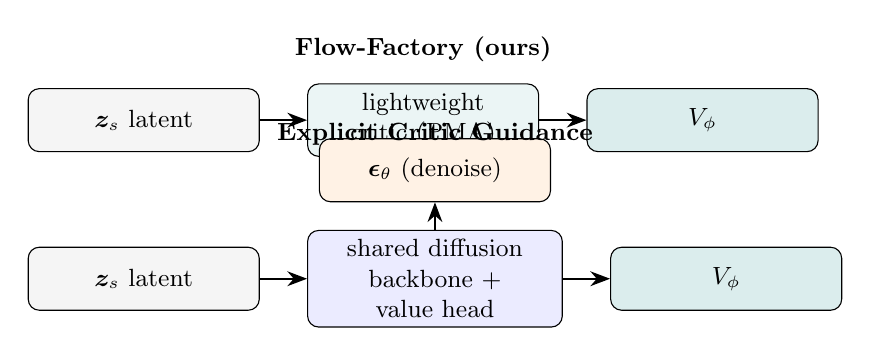
\begin{tikzpicture}[node distance=0.4cm and 0.6cm]
  % Ours
  \node[net, fill=gray!8] (l1) {$\zt_s$ latent};
  \node[net, right=of l1] (c1) {lightweight\\ critic (PMA)};
  \node[net, right=of c1, fill=teal!14] (v1) {$V_\phi$};
  \draw[flow] (l1) -- (c1); \draw[flow] (c1) -- (v1);
  \node[above=0.15cm of c1, font=\small\bfseries] {Flow-Factory (ours)};
  % Paper
  \node[net, fill=gray!8, below=1.2cm of l1] (l2) {$\zt_s$ latent};
  \node[net, right=of l2, fill=blue!8, text width=3.0cm] (c2) {shared diffusion\\ backbone $+$ value head};
  \node[net, right=of c2, fill=teal!14] (v2) {$V_\phi$};
  \node[net, above=0.35cm of c2, fill=orange!10] (eps) {$\bm{\epsilon}_\theta$ (denoise)};
  \draw[flow] (l2) -- (c2); \draw[flow] (c2) -- (v2); \draw[flow] (c2) -- (eps);
  \node[above=0.95cm of c2, font=\small\bfseries] {Explicit Critic Guidance};
\end{tikzpicture}
\caption{Critic body: independent lightweight network (ours) vs.\ the diffusion
backbone reused as its own value function~\cite{liang2026critic}.}
\label{fig:critic-compare}
\end{figure}

\begin{table}[h]
\centering
\small
\begin{tabular}{p{3.1cm} p{5.3cm} p{5.3cm}}
\toprule
\textbf{Aspect} & \textbf{Flow-Factory PPO (ours)} & \textbf{Explicit Critic Guidance~\cite{liang2026critic}} \\
\midrule
Critic body & independent lightweight net; attention-pool on latent tokens & diffusion backbone is its own value function (shared weights $+$ value head) \\
State alignment & $V_\phi(\zt_s,t_s)$ on noisy latent (state-aligned) & value predicted on noisy latent states (state-aligned) \\
Credit assignment & GAE per step & trajectory-level PPO, fine-grained credit \\
Value init & critic warmup (critic-only steps) & value pretraining strategies \\
Inference-time steering & not supported (follow-up) & critic reused for test-time steering (extra gains) \\
Multi-reward & terminal weighted sum; source-aware deferred & joint multi-reward to reduce reward hacking \\
Backbones & model-agnostic (conv / packed / video) & UNet and DiT \\
Cost & cheap: small critic, $O(\mathrm{seq})$ pooling & heavier: a backbone forward per value query \\
\bottomrule
\end{tabular}
\caption{Side-by-side comparison. Both are state-aligned actor--critic PPO for
diffusion; the main axis of difference is the critic body and what it unlocks
(cheap + model-agnostic vs.\ stronger value capacity + inference-time steering).}
\label{tab:compare}
\end{table}

\paragraph{Discussion.}
The paper is strong evidence that the backbone-critic direction pays off, especially
because a shared backbone (i) gives the value head the policy's rich representation,
(ii) conditions on the full prompt/condition for free, and (iii) enables test-time
steering. Flow-Factory's v1 trades some of that value-estimation capacity for a critic
that is essentially free in memory/compute and works across every adapter without
per-architecture surgery. The two designs are complementary: the lightweight critic
is the safe default and reference baseline, while the backbone+value-head critic (and
its inference-time steering and source-aware multi-reward) are the natural next
upgrades, for which this PPO trainer already provides the GAE / dual-optimizer /
checkpoint scaffolding.

\section{Implementation Notes and Configuration}
\label{sec:impl}

\begin{itemize}[leftmargin=1.4em]
  \item \textbf{Files.} \texttt{trainers/ppo/\{critic,gae,trainer\}.py},
  \texttt{hparams/training\_args/ppo.py}, and
  \texttt{models/latent\_geometry.py} (\texttt{compute\_actual\_latent\_shape} /
  \texttt{latent\_shape}). Example: \texttt{examples/ppo/lora/sd3\_5/default.yaml}.
  \item \textbf{Paradigm.} Coupled paradigm: requires SDE dynamics
  (\texttt{Flow-SDE}, \texttt{Dance-SDE}, or \texttt{CPS}). Inherits \texttt{BaseTrainer}.
  \item \textbf{Distributed.} v1 targets DDP (the critic uses a second optimizer);
  DeepSpeed/FSDP support for the second optimizer is a follow-up. The dual-optimizer
  manual-accumulation path is verified for \texttt{bf16}; \texttt{fp16} (a shared
  \texttt{GradScaler} across two optimizers) is a follow-up.
  \item \textbf{Update-frequency decoupling.} \texttt{critic\_update\_interval} /
  \texttt{policy\_update\_interval} (in optimizer rounds) set per-network
  accumulation windows; see \S\ref{sec:decouple}.
  \item \textbf{GAE assumption.} Configure a full, contiguous SDE trajectory
  (\texttt{scheduler.sde\_steps: null}, \texttt{num\_sde\_steps = num\_inference\_steps - 1})
  so the per-step bootstrap is exact.
\end{itemize}

\begin{table}[h]
\centering
\small
\begin{tabular}{lll}
\toprule
Hyperparameter & Default & Meaning \\
\midrule
\texttt{critic\_learning\_rate} & $1\mathrm{e}{-4}$ & critic AdamW LR \\
\texttt{vf\_coef} & $0.5$ & value-loss weight $c_v$ \\
\texttt{gae\_gamma} / \texttt{gae\_lambda} & $1.0$ / $0.95$ & $\gamma$ / $\lambda$ \\
\texttt{value\_clip\_range} & $0.2$ & value clip $\epsilon_v$ (None to disable) \\
\texttt{clip\_range} & $\pm 10^{-4}$ & policy ratio clip $(c_-,c_+)$ \\
\texttt{normalize\_advantage} & true & global advantage whitening \\
\texttt{critic\_warmup\_steps} & $30$ & initial critic-only bootstrap target steps \\
\texttt{critic\_warmup\_interval} & $0$ & periodic re-warmup every $N$ rounds (${\le}0$ off) \\
\texttt{critic\_rewarmup\_steps} & $0$ & target critic steps per periodic re-warmup \\
\texttt{update\_critic\_in\_optimize} & true & false $\Rightarrow$ critic only via warmup/bursts \\
\texttt{critic\_update\_interval} & $1$ & step critic every $N$ rounds \\
\texttt{policy\_update\_interval} & $1$ & step policy every $N$ rounds \\
\texttt{critic\_hidden\_dim} / \texttt{\_num\_layers} & $256$ / $3$ & critic width / depth \\
\texttt{critic\_attn\_heads} / \texttt{\_num\_query\_tokens} & $8$ / $1$ & attention-pool config \\
\texttt{kl\_beta} / \texttt{kl\_type} & $0$ / x-based & optional KL-to-reference \\
\bottomrule
\end{tabular}
\caption{Key \texttt{PPOTrainingArguments} fields.}
\label{tab:hparams}
\end{table}

\section{Limitations and Future Work}
\label{sec:future}

\subsection{Follow-up: DiffAC-style perturbed-state critic training}
\label{sec:perturb-critic}

\paragraph{Idea.}
Today both the \emph{old values} (for GAE) and the in-loop critic regression target
are evaluated on the \emph{rollout} latents the policy actually visited
(\texttt{all\_latents} indexed per SDE step). A cheap, high-leverage upgrade---taken from
DiffAC~\cite{zhou2024diffac}---is to additionally (or alternatively) train the critic on
\emph{forward-perturbed} states: take the generated clean latent $\zt_S$ and re-noise it
to many noise levels $t$ in closed form,
\begin{equation}
\label{eq:perturb}
\zt_t = (1-\sigma_t)\,\zt_S + \sigma_t\,\bm{\epsilon},
\quad \bm{\epsilon}\sim\mathcal N(0,\bm I),\;\; \sigma_t = \texttt{flow\_match\_sigma}(t),
\end{equation}
and regress the critic on each perturbed state toward that sample's terminal reward,
$V_\phi(\zt_t,t)\to R(\zt_S)$ (DiffAC Eq.~8/9). One rollout then yields an
\emph{arbitrarily large}, space-covering set of $(\zt_t,t,R)$ training points instead of
the $S$ sparse on-trajectory states, which lowers value-estimation variance and
improves time coverage. Under the consistency condition (DiffAC Lemma~4.2: when the
backward SDE matches the forward perturbation process, $\zt_t\sim p_{t0}(\cdot\mid\zt_S)$
is distributed as the true rollout marginal $q_t$) these perturbed states are a valid,
on-distribution proxy for the states the GAE consumes.

\paragraph{Why it is cheap here.}
The forward-noising of Eq.~\eqref{eq:perturb} is \emph{already implemented} in the AWM
trainer (\texttt{trainers/awm.py}: \texttt{noised\_latents = (1 - sigma) * clean\_latents
+ sigma * noise}), and the critic forward already accepts an arbitrary
$(\text{latents}, t)$. The change is therefore self-contained.

\paragraph{Plan.}
\begin{enumerate}[leftmargin=1.6em]
  \item \textbf{New hparam} \texttt{critic\_target: \{gae, perturb\_terminal\}} (default
  \texttt{gae}, preserving current behavior), plus \texttt{critic\_perturb\_samples}
  (number of noise levels drawn per clean latent) and a $t$-sampling strategy (reuse
  AWM's \texttt{time\_sampling\_strategy}).
  \item \textbf{Critic training path.} In \texttt{perturb\_terminal} mode, replace the
  rollout-state critic batches in \texttt{\_fit\_critic\_only} (and the in-\texttt{optimize}
  critic branch) with perturbed states from Eq.~\eqref{eq:perturb}, regressed to the
  per-sample terminal reward $R(\zt_S)$ with a \emph{plain} MSE (no cross-step bootstrap;
  this is the $\gamma{=}\lambda{=}1$ Monte-Carlo target). \texttt{\_critic\_value\_loss}
  is reused; \texttt{value\_clip\_range} may be set \texttt{None} to match DiffAC's plain
  MSE.
  \item \textbf{Actor untouched.} The policy still uses PPO-clip; GAE still runs over the
  rollout states, but now bootstraps off a better-calibrated $V_\phi$. (This is the
  variance-reduction half of DiffAC; the full method also moves the \emph{actor} to a
  one-step REINFORCE/DDPG on perturbed states, which is out of scope for this follow-up.)
\end{enumerate}

\paragraph{Caveats to respect.}
\begin{itemize}[leftmargin=1.6em]
  \item \textbf{Monte-Carlo target only.} Perturbed states are mutually independent
  (no ``next'' state), so the critic must regress directly to $R(\zt_S)$; the per-step
  bootstrap of \texttt{compute\_gae} does not apply to these points.
  \item \textbf{Timestep scale.} The $t$ used to noise (Eq.~\eqref{eq:perturb}) and the
  $t$ fed to the critic's time embedding must be on the same scheduler scale, or the
  critic conditions on the wrong noise level.
  \item \textbf{Consistency gap.} The proxy is exact only when the policy stays
  consistent with the forward process; as RL pushes the policy off-distribution the gap
  grows (DiffAC restores it with a score-matching--refit reference; we only borrow the
  critic-side benefit, so treat this as an approximation).
  \item \textbf{Not full DiffAC.} Training only the critic on perturbed states is an
  incremental strengthening of our PPO baseline, not a reproduction of DiffAC.
\end{itemize}

\subsection{Other future work}
\begin{itemize}[leftmargin=1.4em]
  \item \textbf{Backbone+value-head critic} (as in \cite{liang2026critic}): stronger
  value capacity and free conditioning, at $\sim$2$\times$ memory/compute; needs
  per-architecture feature taps. Evaluated and deferred.
  \item \textbf{Inference-time steering} with the learned critic (requires the shared
  backbone).
  \item \textbf{Text / condition conditioning} of the critic (pooled or full prompt
  embeddings) and \textbf{source-aware multi-reward} aggregation.
  \item \textbf{DeepSpeed/FSDP} support for the critic's second optimizer.
\end{itemize}

\begin{thebibliography}{1}
\bibitem{liang2026critic}
Zhengyang Liang, Qihang Zhang, Ceyuan Yang.
\newblock Explicit Critic Guidance for Aligning Diffusion Models.
\newblock arXiv:2605.27736, 2026. \url{https://arxiv.org/abs/2605.27736}

\bibitem{zhou2024diffac}
Xiangxin Zhou, Liang Wang, Yichi Zhou.
\newblock Stabilizing Policy Gradients for Stochastic Differential Equations via
Consistency with Perturbation Process (DiffAC).
\newblock ICML 2024; arXiv:2403.04154. \url{https://arxiv.org/abs/2403.04154}
\end{thebibliography}

\end{document}
